\section{Processing fewer blocks}

The complexity of most demanding on-chain operations of the verifier are linear
to the size of the proof. This includes the proof validation and the evaluation
of score. We now present two techniques that allow for equivalent operations of
constant complexity.

\noindent \textbf{Optimistic schemes.} In smart contracts, in order to ensure that users
comply with the underlying protocol, certain actions are typically
performed on-chain, e.g., verification of data, balance checks, etc. In a
different recently introduced approach, the contract does not perform the
verification initially, but accepts the execution's results at face value.
Actions that deviate from the protocol are reverted only after
honest users indicate them, therefore disallowing them.
Such smart contracts that do not check the validity of actions by default, but
rather depend on the intervention of honest users are characterized
``optimistic''. In the Ethereum community, several projects ~\cite{piza,adler2019building,plasma,rollups-1,rollups-2} have emerged that incorporate the notion of
optimistic interactions. We observe that such an optimization applies to the
NIPoPoW protocol.

We discussed how the verification in the NIPoPoW protocol is realized in two
phases. In the \emph{submit} phase, the verification of $\pis$ is performed.
This is necessary in order to prevent adversaries from submitting structurally
invalid proofs. A proof is \emph{structurally valid} if:
(a) the first block of the proof is the
\emph{genesis} block of the underlying blockchain and
(b) every block has a valid
interlink that points to the previous one in the proof.

Asserting the existence of genesis in the first index of a proof is an
inexpensive operation of constant complexity. However, confirming the interlink
correctness of all blocks is a process of linear complexity to the size of the
proof. Although the verification is performed in memory, sufficiently large
proofs result into costly submissions since their validation constitutes the most
demanding function of the \emph{submit} phase. In
Table~\ref{tab:valid-interlink-cost} we display the cost of the
\textsf{valid-interlink} function which determines the structural correctness
of a proof in comparison with the overall gas used in \textsf{submit}.

\begin{table}[h]
\begin{tabular}{|c|c|c|}
\hline
\textbf{Process} & \textbf{Gas cost} & \multicolumn{1}{l|}{\textbf{Total \%}} \\ \hline
\textsf{verify-interlink} & 2,200,000         & 53\%                                     \\ \hline
\textsf{submit}           & 4,700,000         & 100\%                                    \\ \hline
\end{tabular}
\caption{Gas usage of \textsf{verify-interlink} compared to the overall
gas consumption of \textsf{submit}.}
\label{tab:valid-interlink-cost}
\vspace*{-5mm}
\end{table}


\newcommand{\dispute}{\emph{dispute\ }} \noindent \textbf{Dispute phase.} We
add a new \dispute phase to our protocol. It alleviates the burden of
verifying all elements of the proof by enabling the indication of an individual
incorrect block. This phase allows an honest party to indicate a particular index
where $\pis$ is structurally incorrect. This check takes constant gas.

The process works as follows. Initially, a proof $\pis$ is submitted.
An honest contester monitors the network for proof submissions. This data can be found
in the \texttt{calldata} of a smart contract call transaction. In case
she notices $\pis$ is structurally invalid, she computes the index of the
first block at which it contains an invalid interlink connection. This computation
occurs off-chain.
The contester calls
$\textsf{dispute}$($\pis$, $i$), where $i$
indicates the disputing index of $\pis$. Therefore, the interlink connection between
only two subsequent blocks in the proof is
checked \emph{on-chain} rather than the entire span of $\pis$.

Note that this additional phase does not imply increased rounds of
interactions between the parties. If $\pis$ is invalidated in the
\dispute phase, then the \emph{contest} phase is skipped. Similarly, if
$\pis$ is structurally correct, but represents a dishonest chain, then the contester
proceeds directly to the \emph{contest} phase without invoking of \emph{dispute}.

\begin{table}
\centering
\begin{tabular}{ccccccc|cc}
            & \textbf{Phase} & \textbf{Gas} &  &              & \textbf{Phase} & \textbf{Gas} & \textbf{Phase} & \textbf{Gas} \\ \cline{2-3} \cline{6-9}
 & submit  & 4.7 &  &  & submit  & 2.2 & submit  & 2.2 \\
 & contest & 4.9 &  &  & dispute & 1.3 & contest & 4.9 \\ \cline{2-3} \cline{6-9}
\textbf{I.} & \textbf{Total} & \textbf{9.6} &  & \textbf{II.} & \textbf{Total} & \textbf{3.5} & \textbf{Total} & \textbf{7.1}
\end{tabular}

\caption{Performance per phase. Gas units are displayed in millions.
\textbf{I}: Gas consumption prior to dispute phase incorporation. \textbf{II}:
Gas consumption for two independent sets of interactions submit/dispute and
submit/contest.}

\label{tab:dispute-cost}
\end{table}


In Table~\ref{tab:dispute-cost} we display the gas consumption for
two independent cycles of interactions:
\begin{enumerate}
    \item \emph{Submit} and \emph{dispute} for a structurally invalid
        $\pis$.
    \item \emph{Submit} and \emph{contest} for a structurally valid
        $\pis$ that represents a dishonest chain.
\end{enumerate}

In lines \ref{alg:dispute-best-level:dispute-start}--\ref{alg:dispute-best-level:dispute-end}
of Algorithm~\ref{alg:dispute-best-level}, we show the implementation
of the \emph{dispute} phase. The introduction of the \emph{dispute} phase leaves
\textsf{contest} unchanged.

\noindent \textbf{Isolating the best level.} As we discussed, \emph{dispute}
and \emph{contest} phases are mutually exclusive. Unfortunately, the same
constant-time verification as in the \emph{dispute} phase cannot be applied in a
contest without increasing the rounds of interactions for the users. However,
we derive a subsequent optimization for the \emph{contest} phase by observing the
process of score evaluation.

In NIPoPoWs, after the last common ancestor is found, each proof fork
is evaluated in terms of the proof-of-work score of its blocks after the $\lca$
block. Each level captures a different
score, and the level with the best score for the fork is used for the comparison
(see Algorithm~\ref{alg.nipopow-verifier}).
The position of $\lca$ determines the span of the proofs that
will be included in the score evaluation process. Furthermore, it is impossible
to determine the score of a proof in the \emph{submit} phase because the position
of $\lca$ is yet unknown.

After $\pis$ is retrieved from the calldata, the contester can calculate off-chain
the score of both proofs. This means that the contester knows the level at which each
proof captures the best score for each fork. In light of this
observation, it suffices for the contester to submit the blocks that constitute the \emph{best level}
of $\pic$. The number of these blocks is constant, as it is determined by the
security parameter $m$, which is independent of the size of the underlying
blockchain. We illustrate the blocks that participate in the formulation of a
proof's score and the best level of contesting proof in
Figure~\ref{fig:score-at-levels}.

An adversarial contester can send a level of $\pic$ which is
different than the best. However, this is pointless, since
different levels only undermine her score. On the contrary, due to
the consistency property of \emph{hash-and-resubmit}, $\pis$ cannot be altered.
We denote $b$ the best level of $\pitr$ and the subchain at that level as $\pitrl$.

\begin{figure}
    \centering
    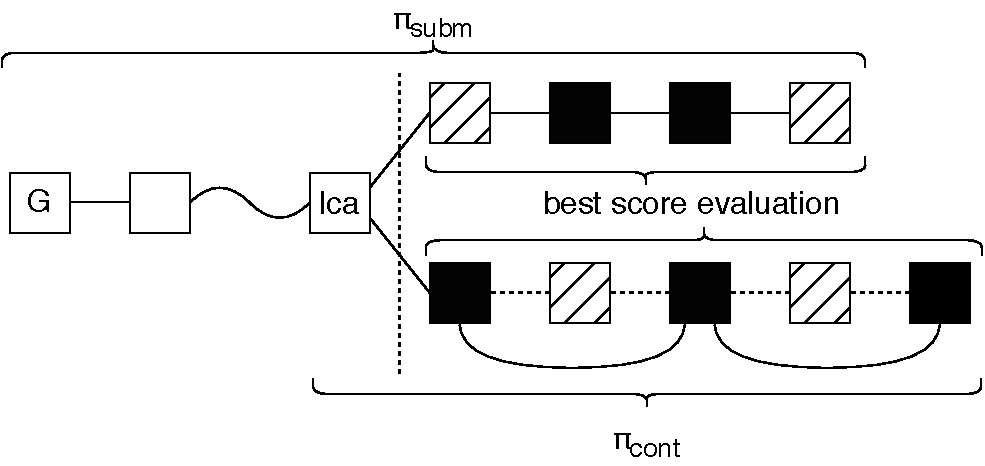
\includegraphics[width=\ourfigurescale\columnwidth]{figures/blocks-of-best-level.pdf}
    \caption{Fork of two proofs. Striped blocks determine the
    score of each proof. Black blocks belong to the level that
    has the best score. Only black blocks are part of the best level of the
    contesting proof.}
    \label{fig:score-at-levels}
\end{figure}

In Algorithm~\ref{alg:dispute-best-level}, we show the implementation of the
\emph{contest} phase under the best-level enhancement. This greatly improves the performance of the client,
because the complexity of the majority of $\textsf{contest}$ functions is
proportional to the size of $\pic$. In Table~\ref{tab:best-level-cost}, we
demonstrate the difference in gas consumption in the various stages of the \emph{contest} phase before and after
using \emph{best-level}. The performance of most functions is improved by
approximately 85\%. This is due to the fact that the size of $\pic$ is
decreased accordingly. For $m=15$, $\pitrl$ consists of 31 blocks, while
$\pitr$ consists of 200 blocks.  Notably, the calculation of score for $\pitrl$
needs 97\% less gas than the na\"ive implementation, because the evaluation of the score of an individual level
is performed entirely in memory.

\begin{table}[]
\begin{tabular}{|c|l|r|r|l|r|r|}
\cline{1-1} \cline{3-4} \cline{6-7}
\textbf{Process} &
   &
  \multicolumn{1}{c|}{\textbf{\begin{tabular}[c]{@{}c@{}}Gas\\ Cost\end{tabular}}} &
  \multicolumn{1}{c|}{\textbf{Total}} &
   &
  \multicolumn{1}{c|}{\textbf{\begin{tabular}[c]{@{}c@{}}Gas\\ Cost\end{tabular}}} &
  \multicolumn{1}{c|}{\textbf{Total}} \\ \cline{1-1} \cline{3-4} \cline{6-7}
  \textsf{valid-interlinks} &            & 900,000   & 18\%  &             & 120,000   & 10\%  \\ \cline{1-1} \cline{3-4} \cline{6-7}
  \textsf{minimal-fork}     &            & 1,900,000 & 39\%  &             & 275,000   & 18\%  \\ \cline{1-1} \cline{3-4} \cline{6-7}
  \textsf{score} (p1)       &            & 750,000   & 16\%  &             & 750,000   & 51\%  \\ \cline{1-1} \cline{3-4} \cline{6-7}
  \textsf{score} (p2)       &            & 950,000   & 19\%  &             & 20,000    & 1\%   \\ \cline{1-1} \cline{3-4} \cline{6-7}
other            &            & 400,000   & 8\%   &             & 300,000   & 20\%  \\ \cline{1-1} \cline{3-4} \cline{6-7}
\textsf{contest}          & \textbf{I} & 4,900,000 & 100\% & \textbf{II} & 1,465,000 & 100\% \\ \cline{1-1} \cline{3-4} \cline{6-7}
\end{tabular}
\caption{Gas usage in contest. I: before utilizing best level. II: after
utilizing best level.}
\label{tab:best-level-cost}
\end{table}


In Figure~\ref{fig:dispute-best-level}, we illustrate the performance gains of
the client using the \emph{dispute} phase and the \emph{best-level} method. The
aggregated gas consumption of the \emph{submit} and \emph{contest} phases is
reduced to {3{,}500{,}000} gas. This makes the contract practical,
since a complete cycle of interactions now effortlessly fits inside a
single Ethereum block.

\begin{algorithm}
    \caption{\label{alg:dispute-best-level}The \textsf{NIPoPoW} client enhanced
        with dispute phase and best-level contesting}

    \begin{algorithmic}[1]

    \Contract{crosschain}
    \State $\textsf{events} \gets \bot;$ $\genesis \gets \bot$
    \Function{\sf initialize}{$\genesis_{remote}$}
        \State $\genesis$ $\gets \genesis_{remote}$
    \EndFunction
    \Function{\sf submit}{$\pis$, $e$}
        \State \textsf{require}($\pis$[0] = $\genesis$)
        \State \textsf{require}($\textsf{events$[e]$} = \bot$)
        \State \textsf{events$[e]$.hash} $\gets$ \textsf{H}($\pis$)
        \State \textsf{events$[e]$.pred} $\gets$
        \textsf{evaluate-predicate}(\textsf{$\pis$}, $e$)
    \EndFunction
    \Function{\sf dispute}{$\pisa$, $e$, $i$}
        \Comment{$i$: dispute index}
        \State \textsf{require}(\textsf{events}$[e]$ $\ne$ $\bot$)
        \State \textsf{require}(\textsf{events$[e]$.hash} $=$ \textsf{H}($\pisa$))
        \State \textsf{require}($\neg \textsf{valid-single-interlink}(\pis, i)$)
        \State \textsf{events$[e]$} $\gets$ $\bot$
    \EndFunction
    \Function{\sf valid-single-interlink}{$\pi$, $i$}
        \State $l\gets\pi[i].\mathsf{level}$
        \If{$\pi[i{+}1].\mathsf{intelink}[l] = \pi[i]$}
        \State \Return true
        \EndIf
        \State \Return false
    \EndFunction
    \Function{\sf contest}{$\pisa$, $\pitrl$, $e$, $f$}
        \State \textsf{require}($\pitrl$[0] = $\pisa[f]$)
        \State \textsf{require}(\textsf{events}$[e]$ $\ne$ $\bot$)
        \State \textsf{require}(\textsf{events$[e]$.hash} $=$ \textsf{H}($\pisa$))
        \State \textsf{require}(\textsf{valid-interlinks}($\pitrl$))
        \State \textsf{require}(\textsf{minimal-fork}($\pisa$,
        $\pitrl$, $f$))
        \State \textsf{require}(\textsf{score-at-level}($\pitrl$)
        $>$ \textsf{score}($\pisa[f{:}]$))
        \State \textsf{events$[e]$.pred} $\gets$
            \textsf{evaluate-predicate}($\pitrl$, $e$)
    \EndFunction
    \Function{\sf score-at-level}{$\pi$}
        \State $l \gets \pi[-1].\textsf{level}$
        \Comment{pick proof level from a block}
        \State $score \gets 0$
        \Comment{set score counter to 0}
        \For{b in $\pi$}
            \State \textsf{require}(b.\textsf{level} = $l$)
            \State $score \gets score {+} 2^l$
        \EndFor
        \State \Return{score}
    \EndFunction
    \EndContract
    \vskip8pt
    \end{algorithmic}
\end{algorithm}



\begin{figure}
    \centering
    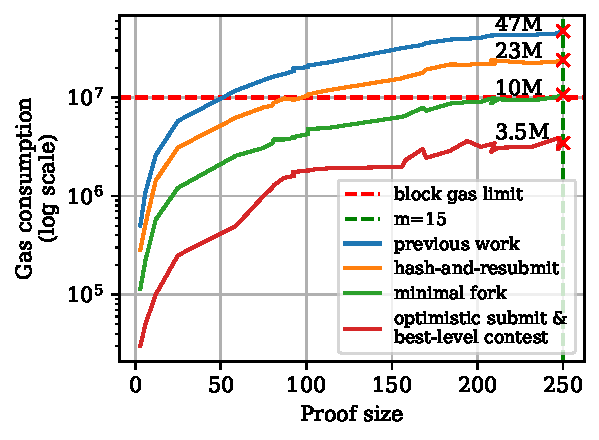
\includegraphics[width=\ourfigurescale\columnwidth]{figures/dispute-best-level.pdf}
    \caption{Performance improvement using \emph{optimistic} evaluation in the submit phase
        and \emph{best level} contestation (lower is better). Gas
        consumption is decreased by approximately 65\%.}
    \label{fig:dispute-best-level}
\end{figure}
